\documentclass[12pt,twoside]{article}
\usepackage{cancel}
\usepackage{physics}
\usepackage{bm}
\usepackage{varioref}
\usepackage{booktabs}
\usepackage{commath}
\usepackage{amsmath}
\usepackage{tikz}
\usepackage{gensymb}

%\usepackage{cite}
\usetikzlibrary{shapes.misc}

\tikzset{cross/.style={cross out, draw=black, minimum size=2*(#1-\pgflinewidth), inner sep=0pt, outer sep=0pt},
%default radius will be 1pt.
cross/.default={1pt}}

\newcommand{\reporttitle}{Midterm exam}
\newcommand{\reportauthor}{}
\newcommand{\reporttype}{}
%\newcommand{\cid}{}

% include files that load packages and define macros
%%%%%%%%%%%%%%%%%%%%%%%%%%%%%%%%%%%%%%%%%
% University Assignment Title Page 
% LaTeX Template
% Version 1.0 (27/12/12)
%
% This template has been downloaded from:
% http://www.LaTeXTemplates.com
%
% Original author:
% WikiBooks (http://en.wikibooks.org/wiki/LaTeX/Title_Creation)
%
% License:
% CC BY-NC-SA 3.0 (http://creativecommons.org/licenses/by-nc-sa/3.0/)
% 
% Instructions for using this template:
% This title page is capable of being compiled as is. This is not useful for 
% including it in another document. To do this, you have two options: 
%
% 1) Copy/paste everything between \begin{document} and \end{document} 
% starting at \begin{titlepage} and paste this into another LaTeX file where you 
% want your title page.
% OR
% 2) Remove everything outside the \begin{titlepage} and \end{titlepage} and 
% move this file to the same directory as the LaTeX file you wish to add it to. 
% Then add \input{./title_page_1.tex} to your LaTeX file where you want your
% title page.
%
%----------------------------------------------------------------------------------------
%	PACKAGES AND OTHER DOCUMENT CONFIGURATIONS
%----------------------------------------------------------------------------------------
\usepackage{ifxetex}
\usepackage{textpos}
\usepackage{natbib}
\usepackage{kpfonts}
\usepackage[a4paper,hmargin=2.8cm,vmargin=2.0cm,includeheadfoot]{geometry}
\usepackage{ifxetex}
\usepackage{stackengine}
\usepackage{tabularx,longtable,multirow,subfigure,caption}%hangcaption
\usepackage{fncylab} %formatting of labels
\usepackage{fancyhdr}
\usepackage{color}
\usepackage[tight,ugly]{units}
\usepackage{url}
\usepackage{float}
\usepackage[english]{babel}
\usepackage{amsmath}
\usepackage{graphicx}
\usepackage[colorinlistoftodos]{todonotes}
\usepackage{dsfont}
\usepackage{epstopdf} % automatically replace .eps with .pdf in graphics
\usepackage{natbib}
\usepackage{backref}
\usepackage{array}
\usepackage{latexsym}
\usepackage{etoolbox}

\usepackage{enumerate} % for numbering with [a)] format 



\ifxetex
\usepackage{fontspec}
\setmainfont[Scale=.8]{OpenDyslexic-Regular}
\else
\usepackage[pdftex,pagebackref,hypertexnames=false,colorlinks]{hyperref} % provide links in pdf
\hypersetup{pdftitle={},
  pdfsubject={}, 
  pdfauthor={\reportauthor},
  pdfkeywords={}, 
  pdfstartview=FitH,
  pdfpagemode={UseOutlines},% None, FullScreen, UseOutlines
  bookmarksnumbered=true, bookmarksopen=true, colorlinks,
    citecolor=black,%
    filecolor=black,%
    linkcolor=black,%
    urlcolor=black}
\usepackage[all]{hypcap}
\fi

\usepackage{tcolorbox}

% various theorems
\usepackage{ntheorem}
\theoremstyle{break}
\newtheorem{lemma}{Lemma}
\newtheorem{theorem}{Theorem}
\newtheorem{remark}{Remark}
\newtheorem{definition}{Definition}
\newtheorem{proof}{Proof}

% example-environment
\newenvironment{example}[1][]
{ 
\vspace{4mm}
\noindent\makebox[\linewidth]{\rule{\hsize}{1.5pt}}
\textbf{Example #1}\\
}
{ 
\noindent\newline\makebox[\linewidth]{\rule{\hsize}{1.0pt}}
}



%\renewcommand{\rmdefault}{pplx} % Palatino
% \renewcommand{\rmdefault}{put} % Utopia

\ifxetex
\else
\renewcommand*{\rmdefault}{bch} % Charter
\renewcommand*{\ttdefault}{cmtt} % Computer Modern Typewriter
%\renewcommand*{\rmdefault}{phv} % Helvetica
%\renewcommand*{\rmdefault}{iwona} % Avant Garde
\fi

\setlength{\parindent}{0em}  % indentation of paragraph

\setlength{\headheight}{14.5pt}
\pagestyle{fancy}
\fancyfoot[ER,OL]{\thepage}%Page no. in the left on
                                %odd pages and on right on even pages
\fancyfoot[OC,EC]{\sffamily }
\renewcommand{\headrulewidth}{0.1pt}
\renewcommand{\footrulewidth}{0.1pt}
\captionsetup{margin=10pt,font=small,labelfont=bf}


%--- chapter heading

\def\@makechapterhead#1{%
  \vspace*{10\p@}%
  {\parindent \z@ \raggedright %\sffamily
        %{\Large \MakeUppercase{\@chapapp} \space \thechapter}
        %\\
        %\hrulefill
        %\par\nobreak
        %\vskip 10\p@
    \interlinepenalty\@M
    \Huge \bfseries 
    \thechapter \space\space #1\par\nobreak
    \vskip 30\p@
  }}

%---chapter heading for \chapter*  
\def\@makeschapterhead#1{%
  \vspace*{10\p@}%
  {\parindent \z@ \raggedright
    \sffamily
    \interlinepenalty\@M
    \Huge \bfseries  
    #1\par\nobreak
    \vskip 30\p@
  }}
  



% %%%%%%%%%%%%% boxit
\def\Beginboxit
   {\par
    \vbox\bgroup
	   \hrule
	   \hbox\bgroup
		  \vrule \kern1.2pt %
		  \vbox\bgroup\kern1.2pt
   }

\def\Endboxit{%
			      \kern1.2pt
		       \egroup
		  \kern1.2pt\vrule
		\egroup
	   \hrule
	 \egroup
   }	

\newenvironment{boxit}{\Beginboxit}{\Endboxit}
\newenvironment{boxit*}{\Beginboxit\hbox to\hsize{}}{\Endboxit}



\allowdisplaybreaks

\makeatletter
\newcounter{elimination@steps}
\newcolumntype{R}[1]{>{\raggedleft\arraybackslash$}p{#1}<{$}}
\def\elimination@num@rights{}
\def\elimination@num@variables{}
\def\elimination@col@width{}
\newenvironment{elimination}[4][0]
{
    \setcounter{elimination@steps}{0}
    \def\elimination@num@rights{#1}
    \def\elimination@num@variables{#2}
    \def\elimination@col@width{#3}
    \renewcommand{\arraystretch}{#4}
    \start@align\@ne\st@rredtrue\m@ne
}
{
    \endalign
    \ignorespacesafterend
}
\newcommand{\eliminationstep}[2]
{
    \ifnum\value{elimination@steps}>0\leadsto\quad\fi
    \left[
        \ifnum\elimination@num@rights>0
            \begin{array}
            {@{}*{\elimination@num@variables}{R{\elimination@col@width}}
            |@{}*{\elimination@num@rights}{R{\elimination@col@width}}}
        \else
            \begin{array}
            {@{}*{\elimination@num@variables}{R{\elimination@col@width}}}
        \fi
            #1
        \end{array}
    \right]
    & 
    \begin{array}{l}
        #2
    \end{array}
    &%                                    moved second & here
    \addtocounter{elimination@steps}{1}
}
\makeatother

%% Fast macro for column vectors
\makeatletter  
\def\colvec#1{\expandafter\colvec@i#1,,,,,,,,,\@nil}
\def\colvec@i#1,#2,#3,#4,#5,#6,#7,#8,#9\@nil{% 
  \ifx$#2$ \begin{bmatrix}#1\end{bmatrix} \else
    \ifx$#3$ \begin{bmatrix}#1\\#2\end{bmatrix} \else
      \ifx$#4$ \begin{bmatrix}#1\\#2\\#3\end{bmatrix}\else
        \ifx$#5$ \begin{bmatrix}#1\\#2\\#3\\#4\end{bmatrix}\else
          \ifx$#6$ \begin{bmatrix}#1\\#2\\#3\\#4\\#5\end{bmatrix}\else
            \ifx$#7$ \begin{bmatrix}#1\\#2\\#3\\#4\\#5\\#6\end{bmatrix}\else
              \ifx$#8$ \begin{bmatrix}#1\\#2\\#3\\#4\\#5\\#6\\#7\end{bmatrix}\else
                 \PackageError{Column Vector}{The vector you tried to write is too big, use bmatrix instead}{Try using the bmatrix environment}
              \fi
            \fi
          \fi
        \fi
      \fi
    \fi
  \fi 
}  
\makeatother

\robustify{\colvec}

%%% Local Variables: 
%%% mode: latex
%%% TeX-master: "notes"
%%% End: 
 % various packages needed for maths etc.
% quick way of adding a figure
\newcommand{\fig}[3]{
 \begin{center}
 \scalebox{#3}{\includegraphics[#2]{#1}}
 \end{center}
}

%\newcommand*{\point}[1]{\vec{\mkern0mu#1}}
\newcommand{\ci}[0]{\perp\!\!\!\!\!\perp} % conditional independence
\newcommand{\point}[1]{{#1}} % points 
\renewcommand{\vec}[1]{{\boldsymbol{{#1}}}} % vector
\newcommand{\mat}[1]{{\boldsymbol{{#1}}}} % matrix
\newcommand{\R}[0]{\mathds{R}} % real numbers
\newcommand{\Z}[0]{\mathds{Z}} % integers
\newcommand{\N}[0]{\mathds{N}} % natural numbers
\newcommand{\nat}[0]{\mathds{N}} % natural numbers
\newcommand{\Q}[0]{\mathds{Q}} % rational numbers
\ifxetex
\newcommand{\C}[0]{\mathds{C}} % complex numbers
\else
\newcommand{\C}[0]{\mathds{C}} % complex numbers
\fi
\newcommand{\tr}[0]{\text{tr}} % trace
\renewcommand{\d}[0]{\mathrm{d}} % total derivative
\newcommand{\inv}{^{-1}} % inverse
\newcommand{\id}{\mathrm{id}} % identity mapping
\renewcommand{\dim}{\mathrm{dim}} % dimension
\newcommand{\rank}[0]{\mathrm{rk}} % rank
\newcommand{\determ}[1]{\mathrm{det}(#1)} % determinant
\newcommand{\scp}[2]{\langle #1 , #2 \rangle}
\newcommand{\kernel}[0]{\mathrm{ker}} % kernel/nullspace
\newcommand{\img}[0]{\mathrm{Im}} % image
\newcommand{\idx}[1]{{(#1)}}
\DeclareMathOperator*{\diag}{diag}
\newcommand{\E}{\mathds{E}} % expectation
\newcommand{\var}{\mathds{V}} % variance
\newcommand{\gauss}[2]{\mathcal{N}\big(#1,\,#2\big)} % gaussian distribution N(.,.)
\newcommand{\gaussx}[3]{\mathcal{N}\big(#1\,|\,#2,\,#3\big)} % gaussian distribution N(.|.,.)
\newcommand{\gaussBig}[2]{\mathcal{N}\left(#1,\,#2\right)} % see above, but with brackets that adjust to the height of the arguments
\newcommand{\gaussxBig}[3]{\mathcal{N}\left(#1\,|\,#2,\,#3\right)} % see above, but with brackets that adjust to the height of the arguments
\DeclareMathOperator{\cov}{Cov} % covariance (matrix) 
\ifxetex
\renewcommand{\T}[0]{^\top} % transpose
\else
\newcommand{\T}[0]{^\top}
\fi
% matrix determinant
\newcommand{\matdet}[1]{
\left|
\begin{matrix}
#1
\end{matrix}
\right|
}



%%% various color definitions
\definecolor{darkgreen}{rgb}{0,0.6,0}

\newcommand{\blue}[1]{{\color{blue}#1}}
\newcommand{\red}[1]{{\color{red}#1}}
\newcommand{\green}[1]{{\color{darkgreen}#1}}
\newcommand{\orange}[1]{{\color{orange}#1}}
\newcommand{\magenta}[1]{{\color{magenta}#1}}
\newcommand{\cyan}[1]{{\color{cyan}#1}}


% redefine emph
\renewcommand{\emph}[1]{\blue{\bf{#1}}}

% place a colored box around a character
\gdef\colchar#1#2{%
  \tikz[baseline]{%
  \node[anchor=base,inner sep=2pt,outer sep=0pt,fill = #2!20] {#1};
    }%
}%
 % short-hand notation and macros

\DeclareRobustCommand{\bigO}{%
  \text{\usefont{OMS}{cmsy}{m}{n}O}%
}

%%%%%%%%%%%%%%%%%%%%%%%%%%%%

\begin{document}
% front page
% Last modification: 2016-09-29 (Marc Deisenroth)
\begin{titlepage}

\newcommand{\HRule}{\rule{\linewidth}{0.5mm}} % Defines a new command for the horizontal lines, change thickness here


%----------------------------------------------------------------------------------------
%	LOGO SECTION
%----------------------------------------------------------------------------------------

%\includegraphics[width = 2.5cm]{./figures/UiO}\\[0.5cm]

\begin{center} % Center remainder of the page

%----------------------------------------------------------------------------------------
%	HEADING SECTIONS
%----------------------------------------------------------------------------------------
\textsc{\LARGE \reporttype}\\[1.5cm]
\textsc{\Large University of Oslo}\\[0.5cm]
\textsc{\large FYS3140 - Mathematical methods in physics}\\[0.5cm]
%----------------------------------------------------------------------------------------
%	TITLE SECTION
%----------------------------------------------------------------------------------------

\HRule \\[0.4cm]
{ \huge \bfseries \reporttitle}\\ % Title of your document
\HRule \\[1.5cm]
\end{center}
%----------------------------------------------------------------------------------------
%	AUTHOR SECTION
%----------------------------------------------------------------------------------------

%\begin{minipage}{0.4\hsize}
\begin{flushleft} \large
\textit{Candidate number: ---}\\
%\reportauthor~(CID: \cid) % Your name
\end{flushleft}
\vspace{2cm}
\makeatletter
Date: \@date

\vfill % Fill the rest of the page with whitespace



\makeatother


\end{titlepage}

\section*{Problem 1: Complex analysis}
\subsection*{Part A: Cauchy integral formula and harmonic functions}
We will begin by studying Cauchy's integral formula for a function $f(z)$ which is analytical inside and on the closed curve $C_R$ defined by
\begin{equation}
  C_R: \abs{z-z_0}=R \label{contour}
\end{equation}
Cauchy's integral formula takes the form
\begin{equation}
  f(z_0) = \frac{1}{2\pi i} \oint_{C_R} \frac{f(z)}{z-z_0}\dif z \label{CIF}
\end{equation}
\subsubsection*{a)}
We let $M$ denote the maximum absolute value of $f(z)$ for all $z$ on the contour $C_R$
\begin{equation}
  \abs{f(z)} \leq M. \label{M}
\end{equation}
We will use this to find an upper bound on the absolute value of $f(z_0)$. To find this value we begin by taking the absolute value on each side of the Cauchy's integral formula \eqref{CIF}
\begin{equation}
  \abs{f(z_0)} = \abs{\frac{1}{2\pi i} \oint_{C_R} \frac{f(z)}{z-z_0}\dif z} = \frac{1}{2\pi}\,\abs{\oint_{C_R} \frac{f(z)}{z-z_0}\dif z}. \label{begining}
\end{equation}
Here we have used that the absolute value of a product is equal to the product of the absolute value of each factor. We continue by writing the absolute value of the integral in terms of a Riemann sum
\begin{equation}
  \abs{\oint_{C_R} \frac{f(z)}{z-z_0}\dif z} = \lim_{n \to \infty} \abs{\sum_{k=1}^{n} \frac{f(z_k)}{z_k-z_0}\Delta z_k}. \label{first_riemann}
\end{equation}
For this sum we will use the generalized triangle inequality, which states that
\begin{equation}
  \abs{\sum_{i}^{n} a_i} \leq \sum_{i}^{n} \abs{a_i}, \label{GTI}
\end{equation}
which is true for an arbitrary number of terms, here denoted $n$. Using the generalized triangle inequality \eqref{GTI} we rewrite the Riemann sum \eqref{first_riemann}
\begin{equation}
  \lim_{n \to \infty} \abs{\sum_{k=1}^{n} \frac{f(z_k)}{z_k-z_0}\Delta z_k} \leq \lim_{n \to \infty} \sum_{k=1}^{n} \abs{\frac{f(z_k)}{z_k-z_0}\Delta z_k} = \lim_{n \to \infty} \sum_{k=1}^{n} \frac{\abs{f(z_k)}}{\abs{z_k-z_0}} \abs{\Delta z_k},
\end{equation}
where we have used that the absolute value of the factors is just the absolute value of each factor. We have already defined an upper bound for $\abs{f(z)}$ equal to $M$ \eqref{M}, and we recognize the denominator as the radius $R$ from the definition of the contour \eqref{contour}. Since both of these are constants we can take them outside of the sum, where we now have a new upper bound estimate
\begin{equation}
  \lim_{n \to \infty} \sum_{k=1}^{n} \frac{\abs{f(z_k)}}{\abs{z_k-z_0}} \abs{\Delta z_k} \leq \frac{M}{R} \,\,\lim_{n \to \infty} \sum_{k=1}^{n} \abs{\Delta z_k}.
\end{equation}
The infinitesimal sums over the changes in $\abs{z_k}$ can not add up to a number larger than the circumference of the curve, which is just a circle with radius $R$. Thus the upper bound of the integral can be written as
\begin{equation}
  \frac{M}{R} \,\,\lim_{n \to \infty} \sum_{k=1}^{n} \abs{\Delta z_k} \leq \frac{M}{R}\,2\pi R.
\end{equation}
We cancel the $R$'s, and tracing the inequalities back to their origin \eqref{first_riemann} leaves us with the simple expression for the upper bound of the integral
\begin{equation}
  \abs{\oint_{C_R} \frac{f(z)}{z-z_0}\dif z} \leq 2\pi M.
\end{equation}
We insert the upper bound of the integral into our original expression for the absolute value of $f(z_0)$ \eqref{begining}
\begin{equation}
  \abs{f(z_0)} = \frac{1}{2\pi}\,\abs{\oint_{C_R} \frac{f(z)}{z-z_0}\dif z} \leq \frac{1}{2\pi} \, 2\pi M.
\end{equation}
Canceling the factors of $2\pi$ we find the final expression for the upper bound estimate for $f$ evaluated at $z_0$
\begin{equation}
  \abs{f(z_0)} \leq M.
\end{equation}

\subsubsection*{b)}
We will try to rewrite Cauchy's integral formula \eqref{CIF} for the special case of a circular contour around a point $z_0$. We do this by writing the complex number $z$ in terms of the center of the circle plus another terms looping around the circle with radius $R$
\begin{equation}
  z = z_0 + R e^{it} \,\,\qquad t \in [0, 2\pi].
\end{equation}
The values chosen for $t$ is a real number such that the exponential term completes one round counter clockwise in the complex plane. By taking the derivative of the new rewrite of $z$ with respect to time we can solve for the infinitesimal $\dif z$
\begin{equation}
  \frac{\dif z}{\dif t} = iRe^{it} \rightarrow \dif z = iRe^{it} \dif t.
\end{equation}
We use this substitution in Cauchy's integral formula \eqref{CIF}
\begin{equation}
  f(z_0) = \frac{1}{2\pi i} \oint_{C_R} \frac{f(z)}{z-z_0}\dif z = \frac{1}{2\pi i} \int_{0}^{2\pi} \frac{f(z_0+Re^{it})}{z_0+Re^{it}-z_0}\,iRe^{it} \dif t.
\end{equation}
We see that the $i$ outside of the integral cancels with the one inside, and by subtracting away the $z_0$'s in the denominator we can cancel the factor $Re^{it}$, leaving us with
\begin{equation}
  f(z_0) = \frac{1}{2\pi} \int_{0}^{2\pi} f(z_0+Re^{it}) \dif t. \label{answer1b}
\end{equation}
This expression will only work for circular contours around $z_0$. We can see that this rewrite gives an easier solution to the previous problem, where we immediately see that $\abs{f(z_0)}$ is bound by the largest value of $f(z)$ along the circle. The factor of $1/2\pi$ outside will cancel with the integral of $\dif t$ from $0$ to $2\pi$ once we factorize out $M$, creating an upper bound for $\abs{f(z_0)}$ equal to $M$.

\subsubsection*{c)}
We introduce the function $u(x, y)$, which is harmonic on and inside a circle of radius $R$ centred at $z_0=x_0+iy_0$. The coordinates of $u(x, y)$ is expressed by a point in the two-dimensional plane, but can equivalently be expressed as a function of a single complex variable $z=x+iy$. All analytic functions can be expressed as a function of a single complex number $z$, and since $u$ is harmonic it has to be analytic. Thus we are allowed to make this change and write $u(x, y)$ as $u(z)$. Since $u(z)$ is analytic we can evaluate it at the center of the circle using Cauchy's integral formula \eqref{CIF}
\begin{equation}
  u(z_0) = \frac{1}{2\pi i} \oint_{C_R} \frac{u(z)}{z-z_0}\dif z.
\end{equation}
In the previous task we showed that such an integral, for a circular contour with radius $R$ around a point $z_0$, can be rewritten to an integral over a real scalar $t$ from $0$ to $2\pi$ \eqref{answer1b}. We use this result, but now for a variable $\theta$ over the same interval, to evaluate $z_0$ at the center of the circle
\begin{equation}
  u(z_0) = \frac{1}{2\pi} \int_{0}^{2\pi} u(z_0+Re^{i\theta}) \dif \theta.
\end{equation}
We are allowed to do this since we have rewritten $u$ to only be a function of a single complex variable, and the fact that $u$ has to be analytic for it to be harmonic.\\
This result tells us that to evaluate an analytic, and in this case harmonic, function at a point $z_0$ we can only use values along a circle of radius $R$ around the given point, and we can do this for a function of two variables as well. Due to the factor $1/2\pi$ outside the integral the function value at the center of the circle is equal to the average value of the function along the contour per angle. It is quite neat that we can do this for an arbitrary radius $R$ (as long as the function is still analytic inside and on the contour), and always be able to evaluate the function at a point we never looked at.

\subsubsection*{d)}
A pair of two-dimensional functions $u(x, y)$ and $v(x, y)$, which are each other's harmonic conjugates, must fulfill
\begin{equation}
  \pdv{u}{x} = \pdv{v}{y} \qquad \qquad \pdv{v}{x} = - \pdv{u}{y}, \label{harmonic_def}
\end{equation}
We can use this to derive the orthogonality of the gradients of the functions $u$ and $v$, where the two-dimensional nabla-operator is defined as
\begin{equation}
  \nabla = \left( \pdv{}{x}, \,\, \pdv{}{y} \right),
\end{equation}
meaning that the inner product between the two functions can be written as
\begin{equation}
  \left( \vec{ \nabla u} \right) \,\cdot   \left( \vec{ \nabla v} \right) = \left( \pdv{u}{x}, \,\, \pdv{u}{y} \right)\cdot \left( \pdv{v}{x}, \,\, \pdv{v}{y} \right) = \pdv{u}{x}\pdv{v}{x} + \pdv{u}{y}\pdv{v}{y}.
\end{equation}
Where we have written the left hand side in bold to emphasis that it is the inner product between two vectors. We then make a substitution from the property of harmonic conjugates \eqref{harmonic_def} on $v$ so that we only have derivatives acting on $u$ in our sum
\begin{equation}
  \left( \vec{ \nabla u} \right) \,\cdot   \left( \vec{ \nabla v} \right) = -\pdv{u}{y}\pdv{u}{x} + \pdv{u}{x}\pdv{u}{y} = 0.
\end{equation}
Since both terms are equal, but with opposite sign, they exactly cancel each other. Thus we have showed that the gradient of two functions which are each others harmonic conjugates have to be orthogonal. We did not specify anything about $u$ and $v$ except from them being harmonic conjugates of each other, thus this orthogonality must hold for all pairs of harmonic conjugates
\begin{equation}
  \left( \vec{ \nabla u} \right) \,\cdot   \left( \vec{ \nabla v} \right) = 0. \label{ortogonality_harmo}
\end{equation}

\subsubsection*{e)}
We will now look at concrete example where one of the harmonic functions, $u(x, y)$, is known, and we want to find it's harmonic conjugate $v(x,y)$. The expression for the known harmonic function is
\begin{equation}
  u(x,y) = \sin{x}\cosh{y}.
\end{equation}
We begin by finding it's derivatives and second derivatives with respect to both $x$ and $y$
\begin{align}
  \begin{split}
  \pdv{u}{x} &= \cos{x}\cosh{y}\qquad \qquad\pdv[2]{u}{x} = -\sin{x}\cosh{y} \\
  \pdv{u}{y} &= \sin{x}\sinh{y}\qquad \qquad\pdv[2]{u}{y} = \sin{x}\cosh{y}. \label{derivatives}
\end{split}
\end{align}
We begin by checking that $u(x, y)$ is in fact harmonic
\begin{equation}
  \nabla^2u = \pdv[2]{u}{x}+\pdv[2]{u}{y} = -\sin{x}\cosh{y} + \sin{x}\cosh{y} = 0,
\end{equation}
here we used the double derivatives calculated in \eqref{derivatives}, and find that $u$ is harmonic. We now want to find the harmonic conjugate of $u$, which we can solve for through the property of harmonic conjugates \eqref{harmonic_def}. We begin with the first equality in \eqref{harmonic_def}, and put in the derivative of $u$ from \eqref{derivatives}
\begin{equation}
  \dv{v}{y} = \dv{u}{x} = \cos{x}\cosh{y}.
\end{equation}
We multiply each side with $\dif y$ and take the integral on both sides
\begin{equation}
  \int \dif v =  \int \cos{x}\cosh{y} \dif y.
\end{equation}
The left hand side will just be the function $v(x, y)$, while on the right hand side we can take $\cos{x}$ outside the integral, and the integral of $\cosh{y}$ is simply $\sinh{y}$, leaving us with
\begin{equation}
  v(x, y) =  \cos{x}\sinh{y} + C(x). \label{first}
\end{equation}
The term $C(x)$ is the integration constant, which can depend on $x$ since we took the integral over $y$. We do get an integration constant on the left hand side, but we can include this in the integration constant $C$ on the right hand side. We repeat the process for the second equality in \eqref{harmonic_def}
\begin{equation}
  \dv{v}{x} = -\dv{u}{y} = - \sin{x}\sinh{y}.
\end{equation}
We multiply each side with $\dif x$ and take the integral
\begin{equation}
  \int \dif v = - \int \sin{x}\sinh{y} \dif x.
\end{equation}
The left hand side will just result in the function $v(x, y)$, while for the right hand side we move $\sinh{x}$ outside and integrate $-\sin{x}$ to $\cos{x}$, thus
\begin{equation}
  v(x, y) = \cos{x}\sinh{y} + C(y). \label{last}
\end{equation}
Where $C(y)$ is the integration constant, which can depend on $y$ since the integral was over $x$.  We do get an integration constant from each side, but these two can be put together to one. The two expressions we have found (\ref{first}, \ref{last}) are consistent with one another, as they should be, and we see that the integration constant can not depend on either $x$ or $y$, and must therefore just be a constant. The final expression $v$ is therefore
\begin{equation}
  v(x, y) = \cos{x}\sinh{y} + C. \label{v}
\end{equation}
Having found both $u(x,y)$ and $v(x,y)$ we can find the analytic function $f=u+iv$, which has the form
\begin{equation}
  f(x, y) = u(x, y) + iv(x, y) = \sin{x}\cosh{y} + i\cos{x}\sinh{y}.
\end{equation}
In our calculations we will ignore the integration constant, as this would only add a constant to the final answer. We begin by writing the trigonometric and hyperbolic functions on exponential form
\begin{equation}
  f(x, y) = \frac{1}{2i}\left(e^{ix}-e^{-ix}\right)\frac{1}{2}\left(e^{y}+e^{-y}\right) + i\frac{1}{2}\left(e^{ix}+e^{-ix}\right)\frac{1}{2}\left(e^{y}-e^{-y}\right).
\end{equation}
We multiply out the parenthesis in each term, and factor out $1/4$
\begin{equation}
  f(x, y) = \frac{1}{4i}\left(e^{ix-y}+e^{ix+y}-e^{-ix-y}-e^{-ix+y}\right) + \frac{i}{4}\left(e^{ix+y}-e^{ix-y}+e^{-ix+y}-e^{-ix-y}\right).
\end{equation}
In the second term we multiply with $i$ in the denominator and numerator, flipping the sign and making the $i$ appear in the denominator so that we can collect the two parenthesis and rewrite the expression to
\begin{equation}
  f(x, y) = \frac{1}{4i}\left(e^{ix-y}+e^{ix+y}-e^{-ix-y}-e^{-ix+y} - e^{ix+y}+ e^{ix-y}-e^{-ix+y}+e^{-ix-y}\right),
\end{equation}
where we see that we have four terms canceling
\begin{equation}
  f(x, y) = \frac{1}{4i}\left(e^{ix-y}+\cancel{e^{ix+y}}-\bcancel{e^{-ix-y}}-e^{-ix+y} - \cancel{e^{ix+y}}+ e^{ix-y}-e^{-ix+y}+\bcancel{e^{-ix-y}}\right),
\end{equation}
leaving us with
\begin{equation}
  f(x, y) = \frac{1}{4i}\left(2e^{ix-y} - 2e^{-(ix-y)}\right).
\end{equation}
We can cancel one factor of $2$ and recognize that we can use $z=x+iy$ to rewrite the exponent as $iz=ix-y$
\begin{equation}
  f(x, y) = \frac{1}{2i}\left(e^{iz} - e^{-iz}\right).
\end{equation}
We recognize this expression as the exponential form of sinus, thus finding the final, simple, form of our function $f$
\begin{equation}
  f(x, y) = \sin{z}.
\end{equation}
If we were to include the integration constant $C$ from our original expression of $v$ \eqref{v} we would find the exact same expression, but including an extra term from the integration constant
\begin{equation}
  f(x, y) = \sin{z} + iC.
\end{equation}
Where the factor $i$ comes from the fact that we begin our calculations from $f=u+iv$, where $v$ contained the integration constant.
\subsubsection*{f)}
Now that we have found a pair of two harmonic conjugates we can test the property of the orthogonality of their gradient \eqref{ortogonality_harmo} found earlier. We begin by calculating their derivatives
\begin{align}
  \begin{split}
  \pdv{u}{x} = \cos{x}\cosh{y}\qquad \qquad\pdv{u}{y} &= \sin{x}\sinh{y} \\
  \pdv{v}{x} = -\sin{x}\sinh{y}\qquad \qquad\pdv{v}{y} &= \cos{x}\cosh{y}. \label{derivatives_2}
\end{split}
\end{align}
The inner product between the two gradients is given by
\begin{equation}
  \left( \vec{ \nabla u} \right) \,\cdot   \left( \vec{ \nabla v} \right) = \left( \pdv{u}{x}, \,\, \pdv{u}{y} \right)\cdot \left( \pdv{v}{x}, \,\, \pdv{v}{y} \right) = \pdv{u}{x}\pdv{v}{x} + \pdv{u}{y}\pdv{v}{y}
\end{equation}
We insert these derivatives into the inner product of the two gradients,
\begin{equation}
  \left( \vec{ \nabla u} \right) \,\cdot   \left( \vec{ \nabla v} \right) = -\cos{x}\cosh{y}\sin{x}\sinh{y} + \sin{x}\sinh{y}\cos{x}\cosh{y} = 0,
\end{equation}
where we see that the two terms are identical, but with opposite sign, and thereby canceling. Our expressions for the harmonic conjugates $u$ and $v$ satisfy the property of orthogonality found previously, as they should.
\subsubsection*{g)}
We have studied the orthogonality of the harmonic conjugates, we will now display this graphically for different functions. We begin with the simple case of
\begin{equation}
  f(z) = x+iy \rightarrow u=x\qquad v=y.
\end{equation}
This is displayed in figure \vref{fig:g1}, where the left most figure is the level curves of $u$, the middle is the level curves of $v$, and the rightmost is both plotted together where $u$ is continuous and $v$ is dashed. In the right most figure we can clearly see the orthogonality as all the dashed and continuous lines cross orthogonally. \par
\begin{figure}
  \centering
  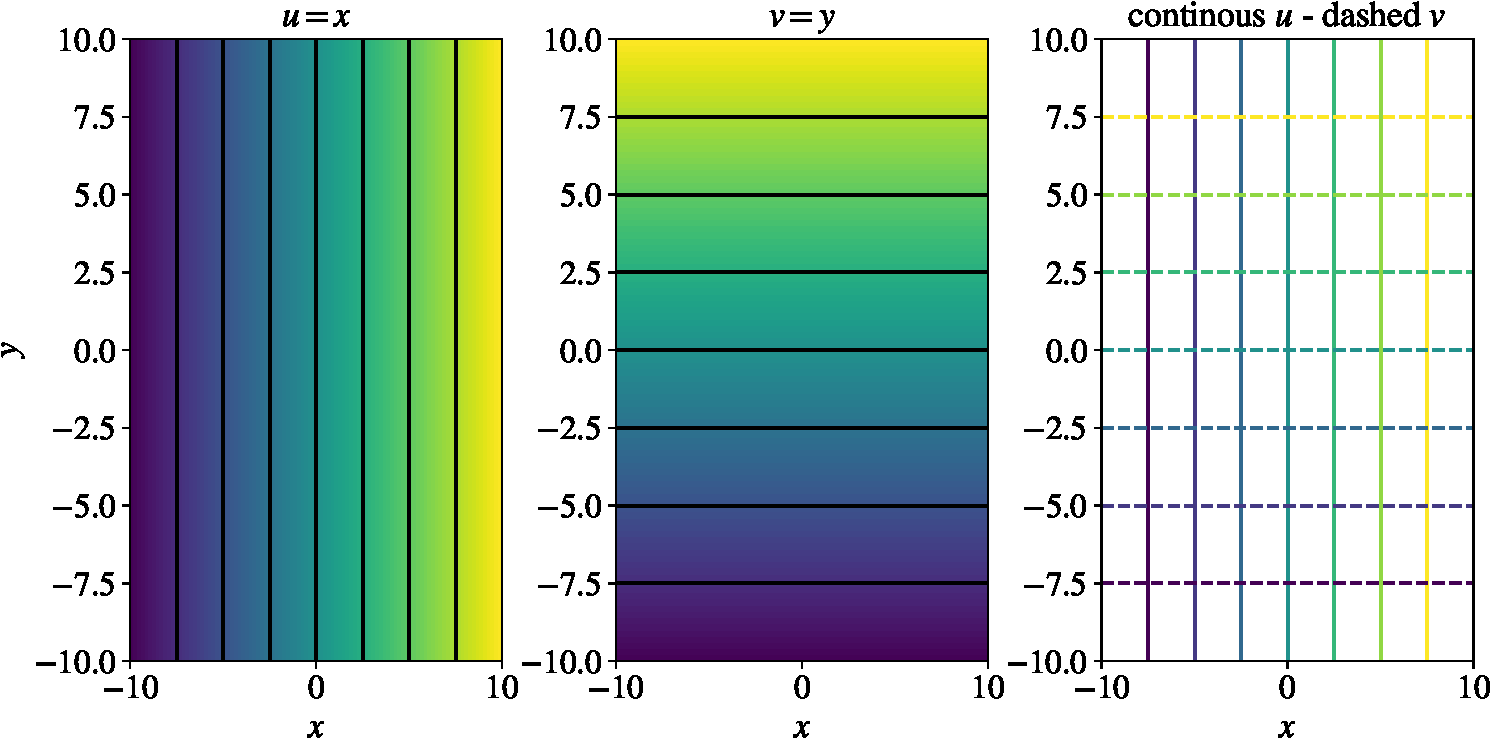
\includegraphics[width=\textwidth]{../figures/first.pdf}
  \caption{The level curves of $u=x$ and $v=y$ is displayed in the left and middle figure respectively, where the colour indicates the function value at a given point, and the black lines show the curves for constant values. The same is true for the last figure, but here we have added the colour to the constant curves. The dashed line is for $v$, and the continuous lines for $u$, we see that the dashed and continuous lines always cross orthogonally.}
  \label{fig:g1}
\end{figure}
We repeat this for the function
\begin{equation}
  f(z) = z^2 = x^2-y^2+2ixy \rightarrow u=x^2-y^2\qquad v=2xy.
\end{equation}
This is displayed in figure \vref{fig:g2}, with the same order as the previous figure. We can again see in the right most figure that the dashed and continuous lines cross orthogonally, as they should do. But we see one exception at the origin where the lines cross at a $45\degree$ angle. I believe this occurs due to limitations of the contour plot numerically, the lines are actually crossing orthogonally, but we have to zoom in to see it. Therefore it is not visible from a distance in our figure, with a finite number of points along the $x$ and $y$ axis.\par
\begin{figure}
  \centering
  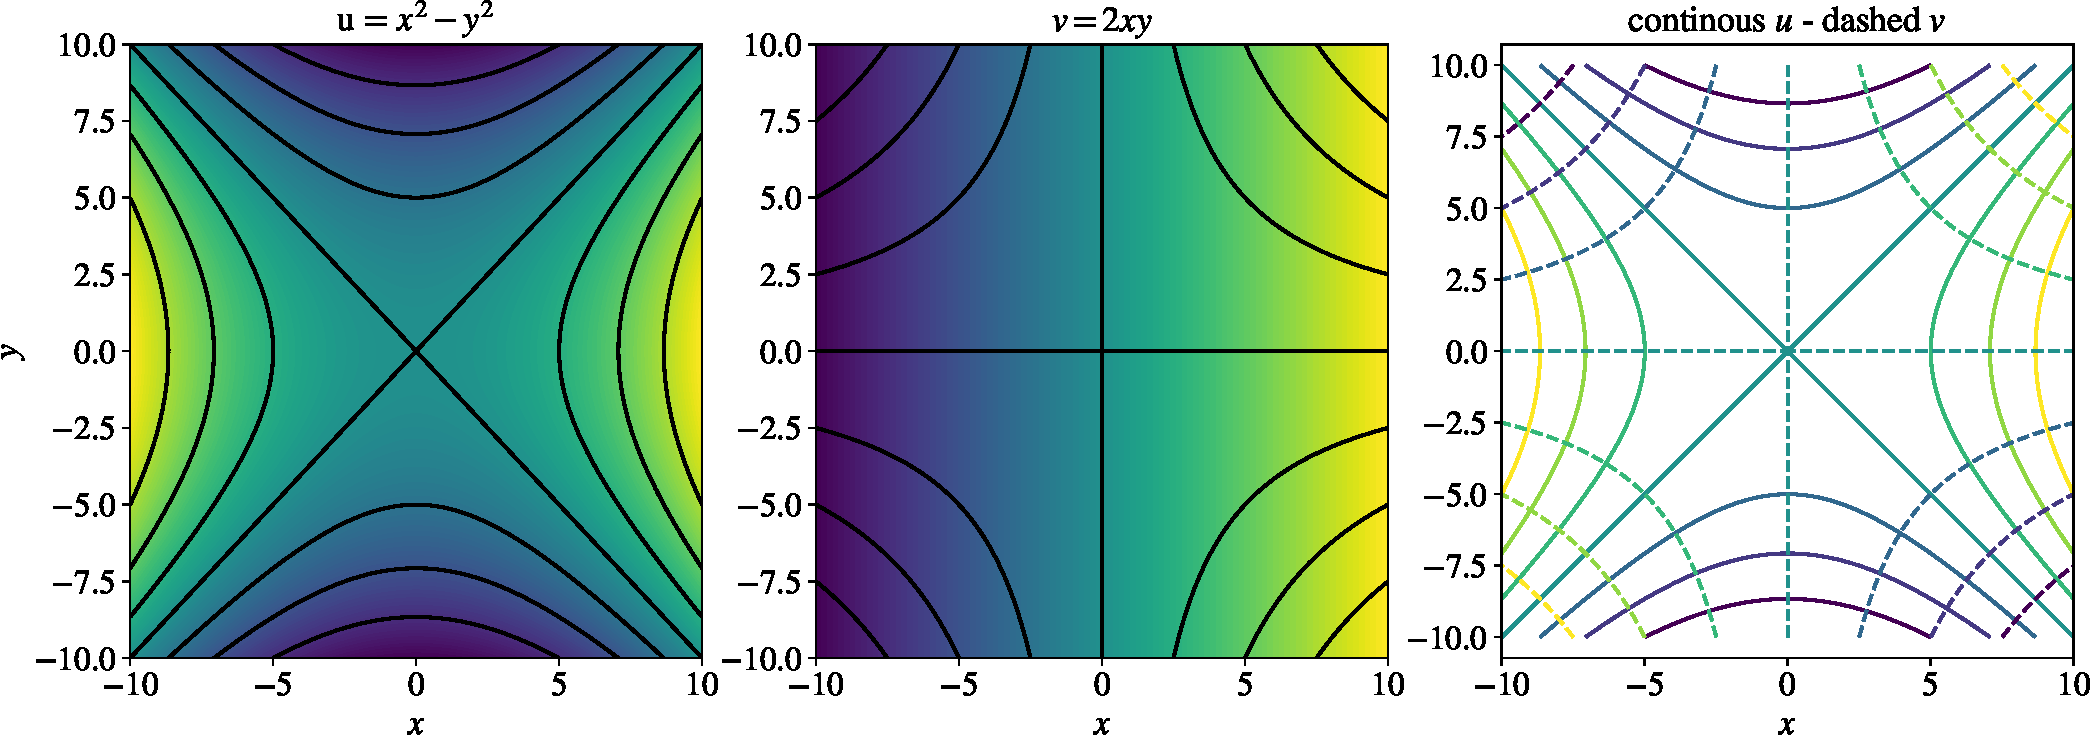
\includegraphics[width=\textwidth]{../figures/secound.pdf}
  \caption{The level curves of $u=x^2-y^2$ and $v=2xy$ is displayed in the left and middle figure respectively, where the colour indicates the function value at a given point, and the black lines show the curves for constant values. The same is true for the last figure, but here we have added the colour to the constant curves. The dashed line is for $v$, and the continuous lines for $u$, we see that the dashed and continuous lines always cross orthogonally.}
  \label{fig:g2}
\end{figure}
Lastly we do this for the function we have just studied
\begin{equation}
  f(z) = \sin{z} = \sin{x}\cosh{y}+i\cos{x}\sinh{y} \rightarrow u=\sin{x}\cosh{y}\qquad v=\cos{x}\sinh{y}.
\end{equation}
This is displayed in figure \vref{fig:g3}, with the same order as the previous figure. We can again see in the right most figure that the dashed and continuous lines cross orthogonally, as they should do.\par
\begin{figure}
  \centering
  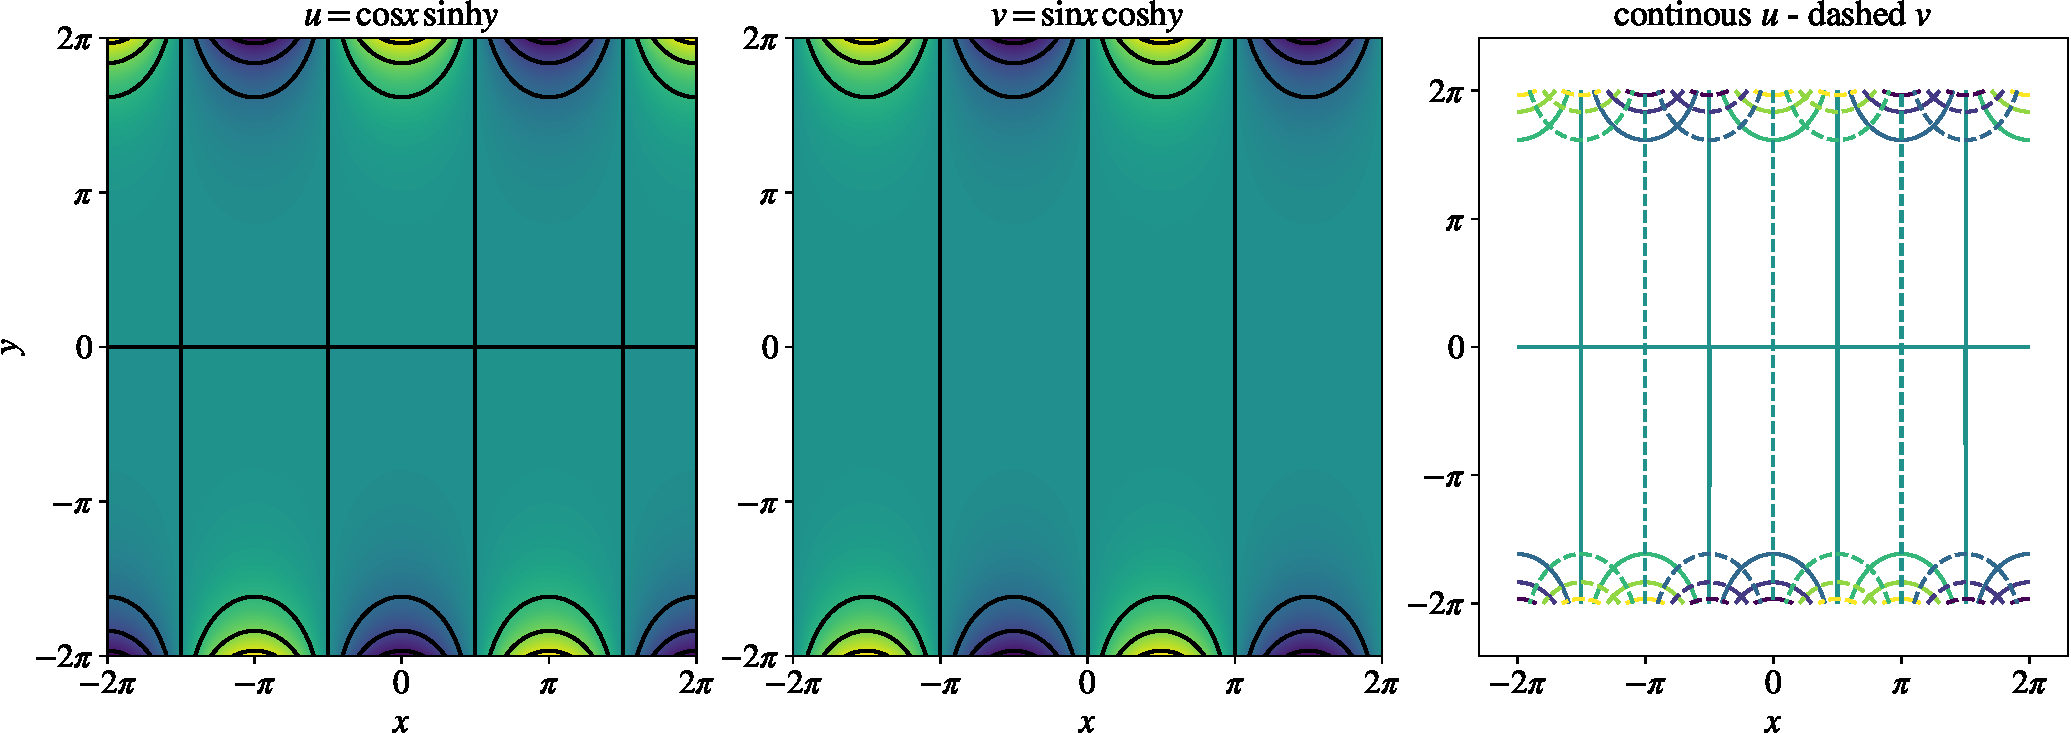
\includegraphics[width=\textwidth]{../figures/third.pdf}
  \caption{The level curves of $u=\sin{x}\cosh{y}$ and $v=\cos{x}\sinh{y}$ is displayed in the left and middle figure respectively, where the colour indicates the function value at a given point, and the black lines show the curves for constant values. The same is true for the last figure, but here we have added the colour to the constant curves. The dashed line is for $v$, and the continuous lines for $u$, we see that the dashed and continuous lines always cross orthogonally.}
  \label{fig:g3}
\end{figure}
For the third graph in all figures we have used \texttt{plt.axis("equal")} in order for the lines to cross orthogonally. Otherwise the axis would be scaled differently such that two lines which were crossing orthogonally would not appear to do so. \\
In the three figures mentioned we see that for the third graph the level curves of $u$ and $v$ always cross orthogonally. Where level curves of a function are the curves in the plane giving a constant value of that function. We know that $\nabla u$ is orthogonal to the level curves of $u$, and the same goes for $v$. Thus when the level curves of $u$ and $v$ cross orthogonally, the gradient of $u$ and $v$ must also be orthogonal. All the level curves shown in figure \ref{fig:g1}, \ref{fig:g2} and \ref{fig:g3} are crossing orthogonally, this is consistent with the orthogonality of the gradients of harmonic conjugates \eqref{ortogonality_harmo} previously derived.

\subsection*{Part B: A contour integral}
\subsubsection*{a)}
We want to solve the contour integral
\begin{equation}
  I = \oint_{C}\frac{4i\left(z^2+4\right)}{z\left(z^2-16\right)}\sin{\left( \frac{5\pi}{z^2+4} \right)} \dif z,
\end{equation}
where $C$ is the closed, circular, curve around $z=3$ with a radius of $2$, $C: \abs{z-3} = 2$. We rewrite the integral by finding the roots of the polynomials to display the singularities more clearly
\begin{equation}
  I = \oint_{C}\frac{4i\left(z+2i\right)\left(z-2i\right)}{z\left(z+4\right)\left(z-4\right)}\sin{\left( \frac{5\pi}{\left(z+2i\right)\left(z-2i\right)} \right)} \dif z. \label{integral}
\end{equation}
With this rewrite we can see that we have singularities at $z=0$, $z=4$ and $z=-4$. We also see that inside the sine we have two points where we divide by zero; $z=2i$ and $z=-2i$. These five points, as well as the curve $C$, is displayed in the complex plane in figure \vref{fig:1Ba}.\par
\begin{figure}
  \centering
  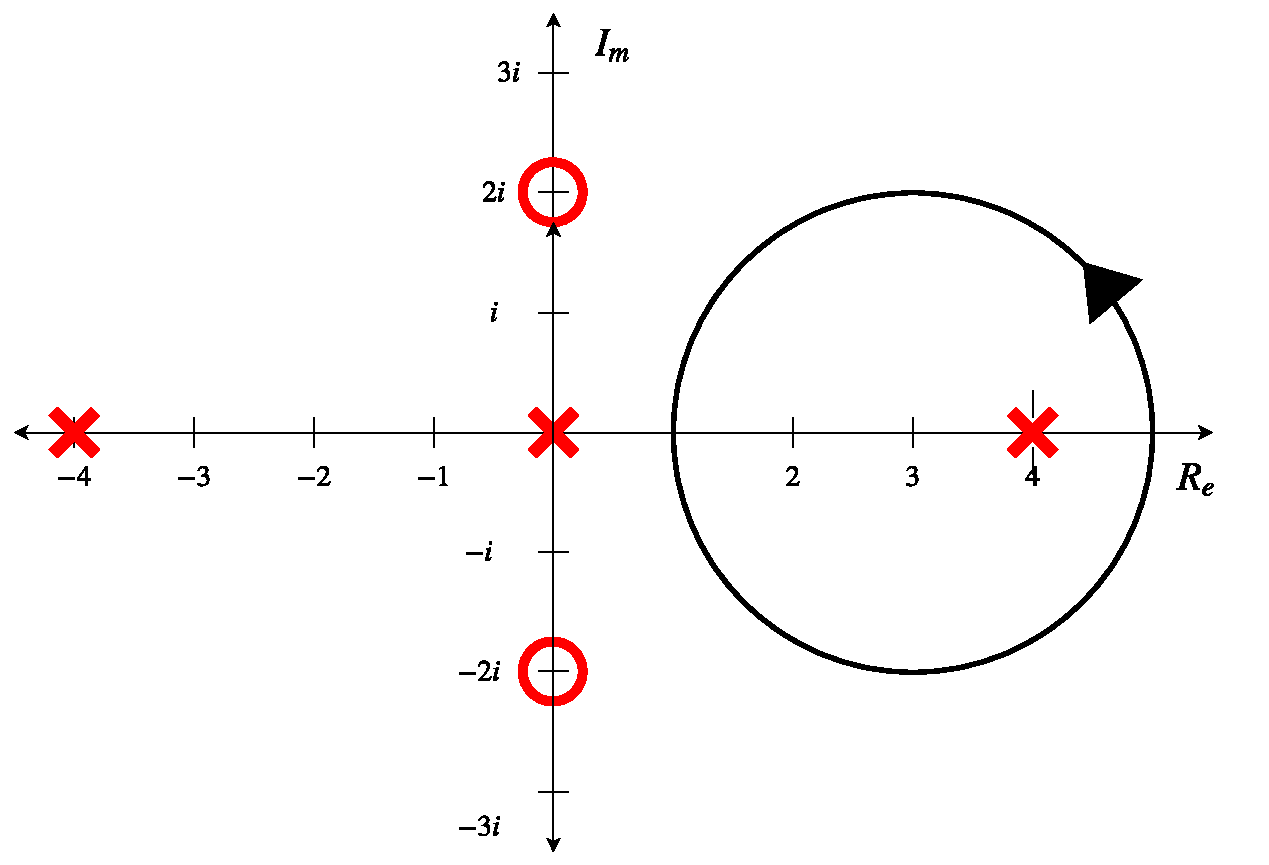
\includegraphics[width=0.8\textwidth]{../figures/contour_and_sing.pdf}
  \caption{The contour $C$ defined as $C: \abs{z-3} = 2$ is shown in the complex plane together with the singularities of our integral \eqref{integral}. The orientation of the contour is shown by the pointing of the arrow. The singularities are displayed as red crosses, while the singularities inside the sine function are displayed as red circles. We see that inside our contour we only have $1$ singularity, which lies at $z=4$.}
  \label{fig:1Ba}
\end{figure}
We see from the figure that there is only one singularity inside the contour, and no singularities on the contour. This singularity is at $z=4$, and we can see that it is a simple pole since it is of order $1$, but we have to be careful to check that this is not a removable singularity. We must check that for $z=4$ the sine factor is not equal to zero, which could have removed the singularity. For $z=4$ the sine-argument is $5\pi/20=\pi/4$, which will make the sine-factor equal to $\sqrt{2}$. Thus the singularity at $z=4$ is not removable.\\
There are many ways to calculate the integral, we could for example use Cauchy's integral formula \eqref{CIF}, or find the integrand's residue at $z=4$. We choose the latter, and find the residue by the following procedure
\begin{equation}
  \text{Res}(z_0) = \lim_{z \to z_0} \left[(z-z_0)f(z)\right],
\end{equation}
where $f(z)$ is the integrand and $z_0$ the singularity we want the residue for. In our case $z_0=4$ and $f(z)$ is the integrand in our integral \eqref{integral}
\begin{equation}
    \text{Res}(4) = \lim_{z \to 4}\left[\cancel{(z-4)}\frac{4i\left(z+2i\right)\left(z-2i\right)}{z\left(z+4\right)\cancel{\left(z-4\right)}}\sin{\left( \frac{5\pi}{\left(z+2i\right)\left(z-2i\right)} \right)}\right].
\end{equation}
We cancel the $(z-4)$ terms, and the value now becomes well defined. We calculate the products and find
\begin{equation}
    \text{Res}(4) = \lim_{z \to 4}\left[\frac{4i\left(z^2+4\right)}{z\left(z+4\right)}\sin{\left( \frac{5\pi}{z^2+4} \right)}\right].
\end{equation}
By evaluating the limit of $z$ we get
\begin{equation}
    \text{Res}(4) = \frac{4i\left(16+4\right)}{4\left(4+4\right)}\sin{\left( \frac{5\pi}{16+4} \right)} = \frac{80i}{32}\sin{\left( \frac{5\pi}{20} \right)} = \frac{5i}{2}\sin{\left(\frac{\pi}{4}\right)} = \frac{5i}{\sqrt{2}}.
\end{equation}
Where we have used that $\sin{\left(\frac{\pi}{4}\right)}=\sqrt{2}$. Since this is the value of the only residue inside our contour we can use it to calculate the integral
\begin{equation}
  I  = 2\pi i\,\,\text{Res}(4) = 2\pi i\frac{5i}{\sqrt{2}} = -5\pi\sqrt{2}
\end{equation}
\newpage
\section*{Problem 2: Variational calculus}
Fermat's principle states that light travels through media with an index of refraction $n$ such that
\begin{equation}
  P = \int n \dif s
\end{equation}
is stationary, where stationary means that the value of the integral is minimized when the integration limits are fixed. In this expression $\dif s$ is an infinitesimal line element, and as we are studying the path of light in a two dimensional plane it is defined as
\begin{equation}
  \dif s = \sqrt{\left(\dif x\right)^2 + \left(\dif y\right)^2}. \label{s}
\end{equation}
We will in this problem assume that the index of refraction is only a function of the $y$-coordinate, $n=n(y)$.
\subsubsection*{a)}
To find the integrand $F$ which makes the integral stationary we will insert the integrand into the Euler-Lagrange equation
\begin{equation}
  \dv{}{t}\left( \dv{F}{\dot{q}} \right) - \dv{F}{q} = 0, \label{EL}
\end{equation}
and solve for one of the coordinates. In this expression $t$ is the integration-variable, and $q$ is the variable of $F$, and $\dot{q}$ is the derivative of $q$ with respect to the integration-variable $t$. With the definition of $\dif s$ \eqref{s} we can either choose to integrate over $x$ or $y$, depending on which one we factorize out of the square root. One option is favorable over the other. We want to choose the integration variable such that one term in the Euler-Lagrange equation \eqref{EL} disappears. Since the index of refraction is only a function of $y$ we see that the right most term in the Euler-Lagrange equation \eqref{EL} will disappear if $q=x$. We will therefore factorize out the $\dif y^2$ in $\dif s$ such that the integrand is only a function of $y$ and $\dot{x}$, where $\dot{x}=\dif x/\dif y$.
Thus we rewrite our integral to the form
\begin{equation}
  P = \int n(y) \sqrt{1+\left(\frac{\dif x}{\dif y}\right)^2} \dif y = \int \underbrace{n(y) \sqrt{1+\dot{x}^2}}_{F} \dif y.
\end{equation}
We put this expression for $F$ into the Euler-Lagrange equation \eqref{EL}, now with $y$ instead of $t$ and $x$ instead of $q$ and see that the second term disappears
\begin{equation}
  \dv{}{y}\left(\dv{}{\dot{x}}\left( n(y) \sqrt{1+\dot{x}^2} \right)\right) - \underbrace{\dv{}{x}\left(n(y) \sqrt{1+\dot{x}^2}\right)}_0 = 0. \label{EL_2}
\end{equation}
Our equation is thereby simplified down to
\begin{equation}
  \dv{}{y}\left(\dv{}{\dot{x}}\left( n(y) \sqrt{1+\dot{x}^2} \right)\right) = 0.
\end{equation}
When the derivative of a function is zero we know that the function must be equal to a constant, which we will call $K$, we can therefore rewrite the equation to
\begin{equation}
  \dv{}{\dot{x}}\left( n(y) \sqrt{1+\dot{x}^2}\right) = K,
\end{equation}
which we want to solve for $\dot{x}$. To do this we begin by calculating the derivative using the chain rule
\begin{equation}
   \frac{n(y)\dot{x}}{\sqrt{1+\dot{x}^2}} = K.
\end{equation}
We divide with the index of refraction before squaring both sides
\begin{equation}
   \frac{\dot{x}^2}{1+\dot{x}^2} = \frac{K^2}{n^2}.
\end{equation}
We divide the the numerator and denominator on the left hand side with $\dot{x}^2$ to only get one term containing $\dot{x}$
\begin{equation}
   \frac{1}{1+\dot{x}^{-2}} = \frac{K^2}{n^2}.
\end{equation}
We flip each fraction and subtract $1$ from each side singling out $\dot{x}^2$
\begin{equation}
   \frac{1}{\dot{x}^{2}} = \frac{n^2}{K^2}-1 = \frac{n^2-K^2}{K^2}.
\end{equation}
We flip the fractions back and take the square root on both sides leaving us with an expression for $\dot{x}$
\begin{equation}
   \dot{x} = \pm\frac{K}{\sqrt{n^2-K^2}}. \label{2a}
\end{equation}
By knowing the derivative of the $x$-coordinate of the light ray as a function of the index of refraction we can determine the path of the light given initial conditions.\\
Since we took the square root we have found both a positive and negative solution for $\dot{x}$. Both solutions are equally correct, as the sign of $\dot{x}$ will be squared inside $F$ anyway. We will in our calculations in this problem use the positive solution, but we could just as well have used the negative one. We will later find that the sign chosen here will enter inside $\cosh{}$, since $\cosh{}$ is a symmetric function around $x=0$ ($\cosh{(-x)}=\cosh{(x)})$ the sign will not matter in our final expression.
\subsubsection*{b)}
We will try and solve equation \eqref{2a} for $y(x)$ to explain the path of light close to the asphalt on a warm day. The closer the air is to the hot asphalt, the hotter the air is. When the air is hotter it becomes less dense, and thereby effecting the index of refraction. We will model this by linearizing the index of refraction
\begin{equation}
  n\left(y\right) = n_0\left(1+\gamma y\right),
\end{equation}
where $\gamma$ is a positive constant with units of one over length. Our coordinate system is set such that $y=0$ corresponds to the ground. From this we see that the index of refraction is equal to $n_0$ on the ground, and increases the further away from the ground you are. We will use this linearization for the index of refraction and solve for the path of the light, starting from \eqref{2a}
\begin{equation}
   \frac{\dif x}{\dif y} = \frac{K}{\sqrt{n_0^2\left(1+\gamma y\right)^2-K^2}}.
\end{equation}
We multiply both sides with $\dif y$ and divide with $K$ upstairs and downstairs on the right hand side
\begin{equation}
   \dif x = \frac{\dif y}{\sqrt{\left(n_0\left(1+\gamma y\right)/K\right)^2-1}}.
\end{equation}
Now we only have $y$ dependence on the right hand side, and $x$ dependence on the left hand side. We can therefore take the integral on each side
\begin{equation}
   \int \dif x = \int \frac{1}{\sqrt{\left(n_0\left(1+\gamma y\right)/K\right)^2-1}} \dif y.
\end{equation}
The left most integral is simply $x$, while to solve the right integral we will begin by substituting away the ugly expression in the denominator
\begin{equation}
  \frac{n_0\left(1+\gamma y\right)}{K} = u \rightarrow \frac{\dif u}{\dif y} = \frac{n_0\gamma}{K} \rightarrow \dif y = \frac{K}{n_0\gamma} \dif u. \label{u}
\end{equation}
We put in for $u$ and $\dif u$ in the integral, becoming
\begin{equation}
   x = \int \frac{1}{\sqrt{u^2-1}} \,\,\frac{K}{n_0\gamma} \dif u,
\end{equation}
Where we can move $K/n_0\gamma$ outside the integral, since they are constants, and multiply them over to the other side of the equal sign. The integral we are left with is therefore simplified down to
\begin{equation}
   \frac{n_0\gamma x}{K} = \int \frac{1}{\sqrt{u^2-1}} \dif u.
\end{equation}
To solve the integral we begin by using a second substitution through $u$
\begin{equation}
  u = \cosh{\xi} \rightarrow \dv{u}{\xi} = \sinh{\xi} \rightarrow \dif u = \sinh{\xi} \, \dif \xi. \label{substitution1}
\end{equation}
We insert this for $u$ and $\dif u$ in the integral
\begin{equation}
   \frac{xn_0\gamma}{K} = \int \frac{\sinh{\xi}}{\sqrt{\cosh^2{(\xi)}-1}} \dif \xi.
\end{equation}
Here we can use the identity of hyperbolic functions
\begin{equation}
\cosh^2{x} -1 = \sinh^2{x}
\end{equation}
to simplify our integral
\begin{equation}
   \frac{xn_0\gamma}{K} = \int \frac{\sinh{\xi}}{\sinh{\xi}} \dif \xi = \int \dif \xi = \xi + C,
\end{equation}
where $C$ is an integration constant.
To find $u$ as a function $\xi$ we use the definition of $\xi$ \eqref{substitution1} and solve for $u$, finding that $\xi = \cosh^{-1}{u}$, giving us
\begin{equation}
   \frac{n_0\gamma x}{K} = \cosh^{-1}{u} + C.
\end{equation}
We do get an integration constant for both integrals, but these two constants can be added together to one. To singel out $u$ we move $C$ over to the other side and take $\cosh{}$ on both sides of the equal sign cancel the inverse, giving us
\begin{equation}
   u = \cosh{\left(\frac{n_0\gamma x}{K}-C\right)}.
\end{equation}
We put in for the definition of $u$ \eqref{u}, and rewrite the expression inside $\cosh{}$
\begin{equation}
   \frac{n_0\left(1+\gamma y\right)}{K} = \cosh{\left(\frac{n_0\gamma}{K}\left(x-\frac{KC}{n_0\gamma}\right)\right)}.
\end{equation}
The new factor containing the integration constant $C$ has unit length, and we will therefore redefine it to
\begin{equation}
  x_0 \equiv \frac{KC}{n_0\gamma} .
\end{equation}
We solve for $y$ and find
\begin{equation}
   y = -\frac{1}{\gamma} + \frac{K}{n_0\gamma}\cosh{\left(\frac{n_0\gamma}{K}\left(x-x_0\right)\right)}.
\end{equation}
Where we have now found an expression for the path of the light ray, where $x_0$ will be determined by the initial conditions. This expression can also be written as
\begin{equation}
   y = \frac{1}{\gamma}\left(\frac{K}{n_0}\cosh{\left(\frac{n_0\gamma}{K}\left(x-x_0\right)\right)}-1\right). \label{2b}
\end{equation}


\subsubsection*{c)}
To simplify the expression for the path of the light we will assume that the argument of $\cosh{}$ is small, such that we can Taylor expand. The first Taylor coefficients of $\cosh{}$ can be shown \cite{Rottmann} to be equal to
\begin{equation}
  \cosh{x}\approx1+\frac{x^2}{2} + \frac{x^4}{24} + \ldots.
\end{equation}
For our expression for $\cosh{}$ \eqref{2b} we will expand around $x=x_0$ such that the derivatives of $\cosh{}$ evaluated at that point is known. In this Taylor expansion we will only include up to the order of $x^3$, and we insert this into our expression for the path of light \eqref{2b}
\begin{equation}
   y = \frac{1}{\gamma}\left(\frac{K}{n_0}\left(1+\frac{1}{2}\left(\frac{n_0\gamma}{K}\left(x-x_0\right)\right)^2 + \bigO\left(\left(\frac{n_0\gamma}{K}\right)^4\right) \right)-1\right)
\end{equation}
By doing the multiplication, and collecting terms with common denominator we can rewrite this expression as
\begin{equation}
   y = \frac{K-n_0}{\gamma n_0} + \frac{n_0\gamma}{2K}\left(x-x_0\right)^2.
\end{equation}
We recognize this expression as a parabola. This solution is shown graphically in figure \vref{fig:2c}. In this figure the axis is scaled such that we do not have to set values for $n_0$, $\gamma$ and $K$. We see that when $x=x_0$ the light ray's altitude is at it's lowest. Thus $x_0$ is the $x-$coordinate corresponding to the minima of the altitude of the light ray, where the path turns around, and begin heading upwards after the decline. The origin of $x_0$ was the integration constant, and thereby the value of $x_0$ is determined through the initial conditions of the light ray.
\begin{figure}[h!]
  \centering
  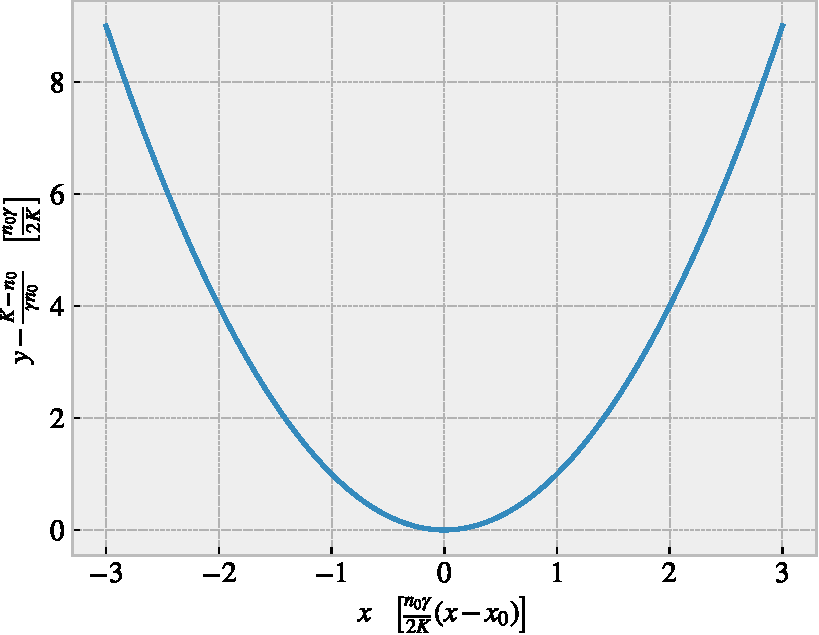
\includegraphics[width=0.575\textwidth]{../figures/2c.pdf}
  \caption{The approximate path of the light ray is displayed for the scaled positions in the $x-y$-plane. We see that the path traces a parabola, where $x=x_0$ is the $x$-position corresponding to the closest altitude to the ground.}
  \label{fig:2c}
\end{figure}
\subsubsection*{d)}
\begin{figure}
  \centering
  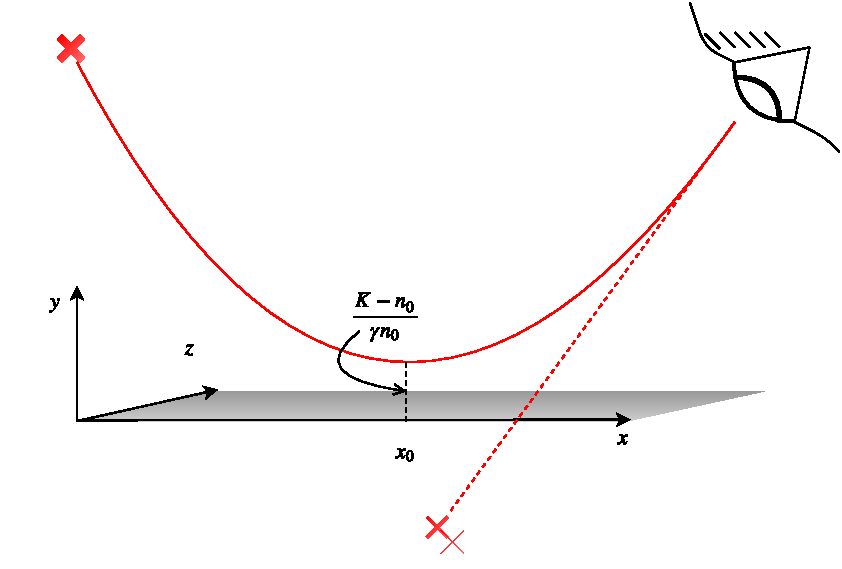
\includegraphics[width=0.67\textwidth]{../figures/drawing.pdf}
  \caption{A qualitative drawing of what will happen when you look at hot asphalt. The red dotted line shows where the object is perceived to be located by the eye. The continuous red line shows the actual path of the light from the position of the object emitting the light. The eye is therefore observing something being \textit{reflected} in the asphalt, even though the light ray never touched the asphalt. In the figure we have indicated the altitude of the minima, which is $(K-n_0)/\gamma n_0$ away from the ground with $x$-coordinate equal to $x_0$. The asphalt is shown spanning in the $z$-direction, while the light ray only moves in the $x-y$-plane.}
  \label{fig:2d}
\end{figure}
We have found an expression for the path of light, but can we use this to explain why the road may look like a mirror on a hot day? When looking down onto the hot asphalt the eye will intercept light which has traveled in the path of the parabola. The eye will therefore see an object in the asphalt which is actually located above. It will look like the light ray was reflected in the asphalt, even though the light ray never touched the asphalt. This is displayed in a qualitative drawing in figure \vref{fig:2d}. This effect is exactly the same as a mirror, we see an object \textit{inside} the mirror, while the actual source of the light is elsewhere.\par
A real world example of this effect, called miraging (luftspeiling), is displayed in figure \vref{fig:2d2}. Here we see that instead of seeing grey asphalt we are actually looking up to the sky. This picture is consistent with what our calculations tell us.
\begin{figure}
  \centering
  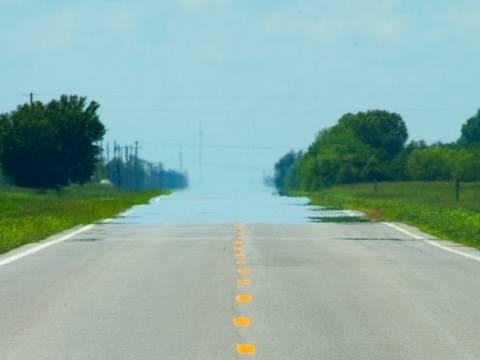
\includegraphics[width=0.7\textwidth]{../figures/picture.jpg}
  \caption{Miraging observed on hot asphalt. Where we expect to see grey asphalt we are actually looking up into the sky. This is due to the bending of the light ray resulting from the temperature dependence on the index of refraction. Image source \cite{sixty_symbols}.}
  \label{fig:2d2}
\end{figure}
%%%%%%%%%%%%%%%%%%%%%%%%%%%% Main document
\newpage
\bibliography{citations.bib}
\bibliographystyle{plain}
\end{document}
